%%%%%%%%%%%%%%%%%%%%%%%%%%%%% Define Article %%%%%%%%%%%%%%%%%%%%%%%%%%%%%%%%%%
\documentclass{article}
%%%%%%%%%%%%%%%%%%%%%%%%%%%%%%%%%%%%%%%%%%%%%%%%%%%%%%%%%%%%%%%%%%%%%%%%%%%%%%%

%%%%%%%%%%%%%%%%%%%%%%%%%%%%% Using Packages %%%%%%%%%%%%%%%%%%%%%%%%%%%%%%%%%%
\usepackage{geometry}
\usepackage{graphicx}
\usepackage{amssymb}
\usepackage{amsmath}
\usepackage{amsthm}
\usepackage{empheq}
\usepackage{mdframed}
\usepackage{booktabs}
\usepackage{lipsum}
\usepackage[export]{adjustbox}
\usepackage{enumitem}
\usepackage{graphicx}
\usepackage{color}
\usepackage{psfrag}
\usepackage{pgfplots}
\usepackage{bm}
\usepackage[spanish]{babel}
%%%%%%%%%%%%%%%%%%%%%%%%%%%%%%%%%%%%%%%%%%%%%%%%%%%%%%%%%%%%%%%%%%%%%%%%%%%%%%%

% Other Settings

%%%%%%%%%%%%%%%%%%%%%%%%%% Page Setting %%%%%%%%%%%%%%%%%%%%%%%%%%%%%%%%%%%%%%%
\geometry{a4paper,margin=1.2in}

%%%%%%%%%%%%%%%%%%%%%%%%%% Define some useful colors %%%%%%%%%%%%%%%%%%%%%%%%%%
\definecolor{ocre}{RGB}{243,102,25}
\definecolor{mygray}{RGB}{243,243,244}
\definecolor{deepGreen}{RGB}{26,111,0}
\definecolor{shallowGreen}{RGB}{235,255,255}
\definecolor{deepBlue}{RGB}{61,124,222}
\definecolor{shallowBlue}{RGB}{235,249,255}
%%%%%%%%%%%%%%%%%%%%%%%%%%%%%%%%%%%%%%%%%%%%%%%%%%%%%%%%%%%%%%%%%%%%%%%%%%%%%%%

%%%%%%%%%%%%%%%%%%%%%%%%%% Define an orangebox command %%%%%%%%%%%%%%%%%%%%%%%%
\newcommand\orangebox[1]{\fcolorbox{ocre}{mygray}{\hspace{1em}#1\hspace{1em}}}
%%%%%%%%%%%%%%%%%%%%%%%%%%%%%%%%%%%%%%%%%%%%%%%%%%%%%%%%%%%%%%%%%%%%%%%%%%%%%%%

%%%%%%%%%%%%%%%%%%%%%%%%%%%% English Environments %%%%%%%%%%%%%%%%%%%%%%%%%%%%%
\newtheoremstyle{mytheoremstyle}{3pt}{3pt}{\normalfont}{0cm}{\rmfamily\bfseries}{}{1em}{{\color{black}\thmname{#1}~\thmnumber{#2}}\thmnote{\,--\,#3}}
\newtheoremstyle{myproblemstyle}{3pt}{3pt}{\normalfont}{0cm}{\rmfamily\bfseries}{}{1em}{{\color{black}\thmname{#1}~\thmnumber{#2}}\thmnote{\,--\,#3}}
\theoremstyle{mytheoremstyle}
\newmdtheoremenv[linewidth=1pt,backgroundcolor=shallowGreen,linecolor=deepGreen,leftmargin=0pt,innerleftmargin=20pt,innerrightmargin=20pt,]{theorem}{Theorem}[section]
\theoremstyle{mytheoremstyle}
\newmdtheoremenv[linewidth=1pt,backgroundcolor=shallowBlue,linecolor=deepBlue,leftmargin=0pt,innerleftmargin=20pt,innerrightmargin=20pt,]{definition}{Definition}[section]
\theoremstyle{myproblemstyle}
\newmdtheoremenv[linecolor=black,leftmargin=0pt,innerleftmargin=10pt,innerrightmargin=10pt,]{problem}{Problem}[section]
%%%%%%%%%%%%%%%%%%%%%%%%%%%%%%%%%%%%%%%%%%%%%%%%%%%%%%%%%%%%%%%%%%%%%%%%%%%%%%%

%%%%%%%%%%%%%%%%%%%%%%%%%%%%%%% Plotting Settings %%%%%%%%%%%%%%%%%%%%%%%%%%%%%
\usepgfplotslibrary{colorbrewer}
\pgfplotsset{width=8cm,compat=1.9}
%%%%%%%%%%%%%%%%%%%%%%%%%%%%%%%%%%%%%%%%%%%%%%%%%%%%%%%%%%%%%%%%%%%%%%%%%%%%%%%

%%%%%%%%%%%%%%%%%%%%%%%%%%%%%%% Title & Author %%%%%%%%%%%%%%%%%%%%%%%%%%%%%%%%
\title{Certamen 1 Introducción a la prospección remota}
\author{Alex Villarroel Carrasco}
%%%%%%%%%%%%%%%%%%%%%%%%%%%%%%%%%%%%%%%%%%%%%%%%%%%%%%%%%%%%%%%%%%%%%%%%%%%%%%%

\begin{document}
\usetikzlibrary{positioning}
	\tikzset{every picture/.style={line width=0.75pt}}    
	\pagestyle{plain}
	\begin{flushleft}
		Departamento de Geofísica \hfill Introducción a prospección geofísica\\
		Facultad de Cs. Físicas y Matemáticas\\
		\underline{Universidad de Concepción}
	\end{flushleft}
	
	\begin{flushright}\vspace{-5mm}
		
\includegraphics[height=1.5cm]{escudo.png}
	\end{flushright}
	
	\begin{center}\vspace{-1cm}
		\textbf{\large Certamen 01 de introducción a prospección geofísica}\\
		{\textcolor{blue}{Alex Villarroel Carrasco}}\\
	\end{center}
	\rule{\linewidth}{0.1mm}
	\\
    \section*{Pregunta 1}
	 1. De las imágenes respectivas para cada caso (2 casos: 1\_PELEHUE y 10\_PELEHUE)
		“picar” una primera llegada para cada geófono, siempre que resulte adecuado
		hacerlo. Construir una tabla con tiempo vs d istancia. Recordar considerar la
		distancia igual a cero (0) el punto del “shot point” respectivo.
	\section*{Respuesta}
	A partir de los archivos entregados por el profesor, se realizó el manejo de datos mediante Obspy, para rehacer un plot de distancia vs tiempo(script adjuntado en Anexos).
	.\par
	\begin{figure}[h]
		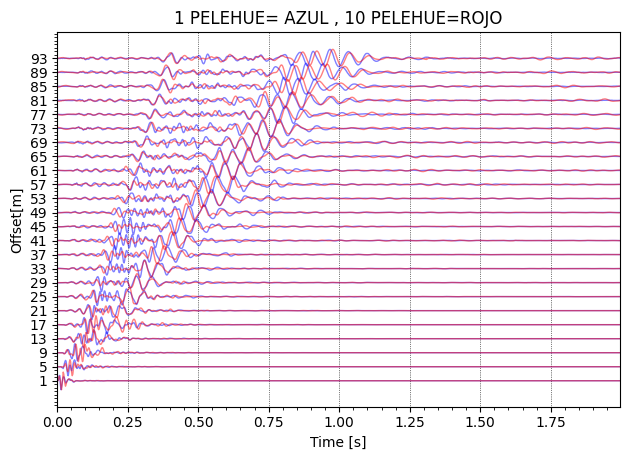
\includegraphics[width=\textwidth]{ambos.png}
		\caption[]{Figura Tiempo-Distancia de cada sismograma para ambos eventos(1 PELEHUE Y 10 PELEHUE)}
	\end{figure}
	Luego de aquello, el picado de la primera llegada se logró mediante la utilización de \textbf{SeisGram2K}, obteniendo las siguientes figuras.
	\begin{figure*}[h]
		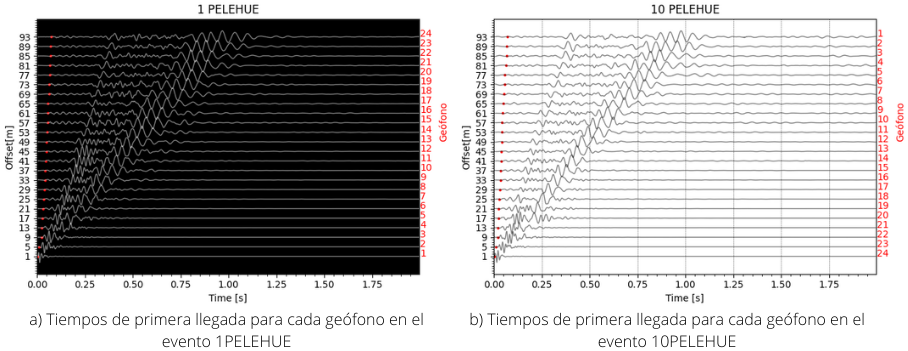
\includegraphics[width=1.3\textwidth,center]{/home/alex/Prospeccion-geofisica/Cert1/fig1.png}
		\caption{Tiempos de primera llegada para cada sismograma. $a)$ correspondiente al evento 1PELEHUE, $b)$ correspondiente al evento 10 PELEHUE}
	\end{figure*}


	\newpage
	Visualmente no se logra apreciar con exactitud los tiempos de llegada en cada geófono, por lo que se presenta una tabla con aquellos datos.
	\\% Please add the following required packages to your document preamble:
	\begin{table}[h!]
		\centering
		\begin{tabular}{|c|c|c|}
		\hline
		\textbf{Geofono} & \textbf{Distancia {[}m{]}} & \textbf{Tiempo {[}s{]}} \\ \hline
		1                & 1                          & 0.002                   \\ \hline
		2                & 5                          & 0.012                   \\ \hline
		3                & 9                          & 0.024                   \\ \hline
		4                & 13                         & 0.024                   \\ \hline
		5                & 17                         & 0.03                    \\ \hline
		6                & 21                         & 0.032                   \\ \hline
		7                & 25                         & 0.037                   \\ \hline
		8                & 29                         & 0.04                    \\ \hline
		9                & 33                         & 0.042                   \\ \hline
		10               & 37                         & 0.043                   \\ \hline
		11               & 41                         & 0.045                   \\ \hline
		12               & 45                         & 0.048                   \\ \hline
		13               & 49                         & 0.051                   \\ \hline
		14               & 53                         & 0.052                   \\ \hline
		15               & 57                         & 0.056                   \\ \hline
		16               & 61                         & 0.058                   \\ \hline
		17               & 65                         & 0.058                   \\ \hline
		18               & 69                         & 0.063                   \\ \hline
		19               & 73                         & 0.064                   \\ \hline
		20               & 77                         & 0.066                   \\ \hline
		21               & 81                         & 0.068                   \\ \hline
		22               & 85                         & 0.07                    \\ \hline
		23               & 89                         & 0.072                   \\ \hline
		24               & 93                         & 0.073                   \\ \hline
		\end{tabular}
		\caption{Tabla de tiempo de llegada para cada geófono en el evento 1PELEHUE}
		\end{table}
		\begin{table}[h!]
			\centering
			\begin{tabular}{|c|c|c|}
			\hline
			\textbf{Geofono} & \textbf{Distancia {[}m{]}} & \textbf{Tiempo {[}s{]}} \\ \hline
			24               & 1                          & 0.004                   \\ \hline
			23               & 5                          & 0.012                   \\ \hline
			22               & 9                          & 0.021                   \\ \hline
			21               & 13                         & 0.022                   \\ \hline
			20               & 17                         & 0.025                   \\ \hline
			19               & 21                         & 0.025                   \\ \hline
			18               & 25                         & 0.027                   \\ \hline
			17               & 29                         & 0.031                   \\ \hline
			16               & 33                         & 0.035                   \\ \hline
			15               & 37                         & 0.036                   \\ \hline
			14               & 41                         & 0.039                   \\ \hline
			13               & 45                         & 0.04                    \\ \hline
			12               & 49                         & 0.043                   \\ \hline
			11               & 53                         & 0.044                   \\ \hline
			10               & 57                         & 0.044                   \\ \hline
			9                & 61                         & 0.046                   \\ \hline
			8                & 65                         & 0.05                    \\ \hline
			7                & 69                         & 0.053                   \\ \hline
			6                & 73                         & 0.055                   \\ \hline
			5                & 77                         & 0.058                   \\ \hline
			4                & 81                         & 0.063                   \\ \hline
			3                & 85                         & 0.066                   \\ \hline
			2                & 89                         & 0.069                   \\ \hline
			1                & 93                         & 0.072                   \\ \hline
			\end{tabular}
			\caption{Tabla de tiempo de llegada para cada geógono en el evento 10PELEHUE}

		\end{table}
	\newpage
	\section*{Curvas camino-tiempo}
	\newpage
	Al extraer los datos y realizar un gráfico de curvas camino-tiempo, se obtuvo lo siguiente:\par
	\begin{figure*}[h!]
		\centering
		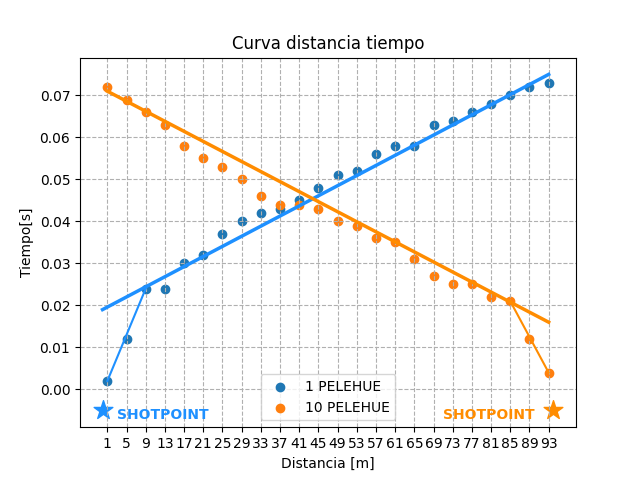
\includegraphics[width=\textwidth,center]{CurvaDist-tiempo.png}
		\caption[]{Curvas camino-tiempo de ambos eventos, con sus respectivas rectas }
	\end{figure*}
	En la figura se aprecia que en ambos eventos existen 2 rectas, la primera correspondiendo a la primera llegada de una onda directa, mientras que la otra recta corresponde a la onda refractada
	.\par La obtención de estas rectas están representadas por las siguientes ecuaciones:
	\subsection*{Evento 1 PELEHUE}
	\begin{enumerate}
		\item Onda directa: \begin{equation*}
			T=0 + 0.023D
			\end{equation*}
			Correspondiendo 0 al intercepto y 0.023 la pendiente de la recta. Es interesante notar que el intercepto debe ser 0 debido a que 
			cuando en un principio si se tuviera a un geofono a 0 metros del shotpoint, demoraría 0 segundos en registrar la llegada(lo cual me parece improbable debido a la precisión y delay que presenta el instrumento)
		\item Onda refractada:\begin{equation*}
			T=\tau+m\cdot D
		\end{equation*}
		Si bien estas rectas pueden ser descritas mediante software, una forma sencilla es tomar dos puntos
		y calcular la pendiente m como $\frac{y_2-y_1}{x_2-y_1}$ y el intercepto despejandolo con los valores conocidos.
		.\par Sea $x_1=9,y_1=0.24$ y $x_2=89,y_2=0.72$  
		\begin{align*}
			m&=\frac{y_2-y_1}{x_2-x_1} \\
			m&=\frac{0.072-0.024}{89-9}\\ 
			m&=0.0006
		\end{align*}
		El intercepto $\tau:$ puede ser obtenido con el punto $(x_1,y_1)$
		\begin{align*}
			y_1&=\tau+0.0006x_1 \\
			\tau&=y_1-0.0006x_1 \\
			\tau&=0.024-0.0006\cdot 9 \\
			\tau&=0.018
		\end{align*}
		por lo que la ecuación de la recta para la onda refractada queda:
		\begin{equation*}
			T=\tau+0.0006D
		\end{equation*}
		con $\tau=0.018$
	\end{enumerate}
	\subsection*{Evento 10 PELEHUE}
	Realizando el mismo procedimiento que antes:
	\begin{enumerate}
		\item Onda directa: \par 
		Teniendo $(x_1,y_1)=(1,0.004)$ y $(x_2,y_2)=(9,0.021)$, y m como $\frac{y_2-y_1}{x_2-y_1}$
		, se tiene la siguiente ecuación de la recta:
		\begin{equation*}
			T=0 + 0.0022D
			\end{equation*}
			Correspondiendo 0 al intercepto y 0.023 la pendiente de la recta. Es interesante notar que el intercepto debe ser 0 debido a que 
			cuando en un principio si se tuviera a un geofono a 0 metros del shotpoint, demoraría 0 segundos en registrar la llegada(lo cual me parece improbable debido a la precisión y delay que presenta el instrumento)
		\item Onda refractada:\begin{equation*}
			T=\tau+m\cdot D
		\end{equation*}
		Se puede calcular la pendiente m como $\frac{y_2-y_1}{x_2-y_1}$ y el intercepto despejandolo con los valores conocidos.
		.\par Sea $x_1=9,y_1=0.021$ y $x_2=89,y_2=0.069$  
		\begin{align*}
			m&=\frac{y_2-y_1}{x_2-x_1} \\
			m&=\frac{0.069-0.021}{89-9}\\ 
			m&=0.0006
		\end{align*}
		El intercepto $\tau:$ puede ser obtenido con el punto $(x_1,y_1)$
		\begin{align*}
			y_1&=\tau+0.0006x_1 \\
			\tau&=y_1-0.0006x_1 \\
			\tau&=0.021-0.0006\cdot 9 \\
			\tau&=0.016
		\end{align*}
		por lo que la ecuación de la recta para la onda refractada queda:
		\begin{equation*}
			T=\tau+0.0006D
		\end{equation*}
		con $\tau=0.016$
	\end{enumerate}
\subsection*{Modelo de estructura-velocidad 1-D (para cada caso)}
Se sabe que la pendiente m calculada anteriormente es el inverso de la velocidad, por lo que se puede extraer la velocidad de la onda directa y reflectada para cada caso.
\begin{itemize}
	\item 1 PELEHUE:\begin{itemize}
		\item Onda directa:\begin{align*}
			V_0&=\frac{1}{m}=\frac{1}{0.0023}\\
			V_0&=435\left[\frac{m}{s}\right]
		\end{align*}
		\item Onda refractada\begin{align*}
			V_1&=\frac{1}{m}=\frac{1}{0.0006}\\
			V_1&=1667\left[\frac{m}{s}\right]
		\end{align*}
	\end{itemize}
	%
	%
	\item 10 PELEHUE:\begin{itemize}
		\item Onda directa:\begin{align*}
			V_0&=\frac{1}{m}=\frac{1}{0.0022}\\
			V_0&=454\left[\frac{m}{s}\right]
		\end{align*}
		\item Onda refractada\begin{align*}
			V_1&=\frac{1}{m}=\frac{1}{0.0006}\\
			V_1&=1667\left[\frac{m}{s}\right]
		\end{align*}
	\end{itemize}
\end{itemize}
\subsection*{Modelo estructura-velocidad}
Para un modelo de una capa no inclinada, el tiempo se puede expresar como función del ángulo crítico, la distancia vertical y horizontal, y de la velocidad, de la siguiente forma:
\begin{equation*}
	T=2z\frac{cos(i_c)}{V}+\frac{x}{V}
\end{equation*}
lo cual se puede extender a:\begin{equation*}
	T_r=\frac{x}{V_2}+2z_1\left(\frac{1}{V_1^2}-\frac{1}{V_2^2}\right)^\frac{1}{2}
\end{equation*}
es fundamental entender que ya se conoce la ecuación de la recta,
y por consiguiente $\tau$, que corresponde al término $2z_1{\left(\frac{1}{V_1^2}-\frac{1}{V_2^2}\right)}^{\frac{1}{2}}$
, pudiendo así extraer $z_1$.
\subsubsection*{1-Pelehue}
\begin{align*}
	\tau&=2z_1\left(\frac{1}{V_1^2}-\frac{1}{V_2^2}\right)^\frac{1}{2}\\ 
	0.018&=2z_1\left(\frac{1}{435^2}-\frac{1}{1667^2}\right)^\frac{1}{2} \\ 
	0.018&=2z_1\cdot 0.0023\\
	z_1&=\frac{0.018}{2\cdot 0.0024}=3.7 [m]
\end{align*}
Para el shotpoint realizado a un metro del geófono 1, el perfil sería el siguiente:
\begin{figure*}
	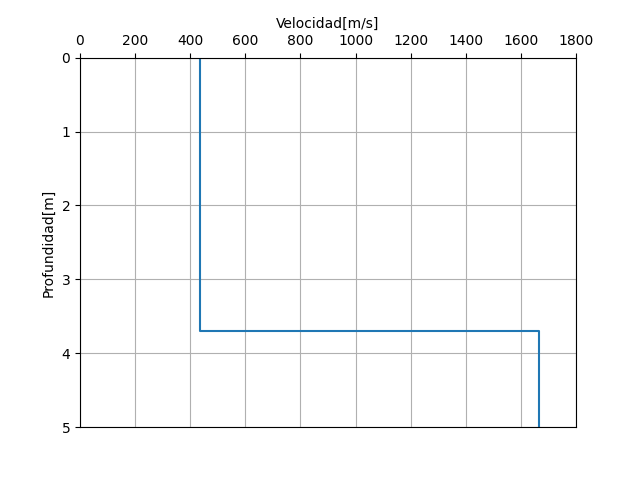
\includegraphics[width=0.8\textwidth,center]{vel-depth.png}
	\caption{Modelo 1-D estructura-velocidad para el evento 1 PELEHUE}
\end{figure*}
\subsubsection*{10-Pelehue}
\begin{align*}
	\tau&=2z_1\left(\frac{1}{V_1^2}-\frac{1}{V_2^2}\right)^\frac{1}{2}\\ 
	0.016&=2z_1\left(\frac{1}{454^2}-\frac{1}{1667^2}\right)^\frac{1}{2} \\ 
	0.016&=2z_1\cdot 0.0022\\
	z_1&=\frac{0.016}{2\cdot 0.0022}=3.5 [m]
\end{align*}
Para el shotpoint realizado a un metro del geófono 24, el perfil sería el siguiente:
\par \begin{figure*}[h!]
	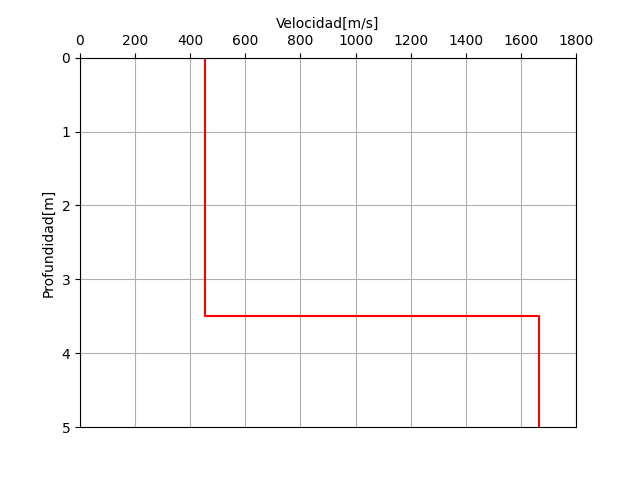
\includegraphics[width=1\textwidth,center]{vel-depth2.png}
	\caption{Modelo 1-D estructura-velocidad para el evento 10 PELEHUE}
\end{figure*}\newpage
\subsection*{¿Capa inclinada o no?}
A partir de los tiempos de las primeras llegadas, de las ecuaciones de recta 
para cada caso, y del modelo 1-D de estructura-velocidad, se puede concluir que no se trata 
de una capa inclinada, ya que las diferencias entre cada evento son ínfimas, 
y pueden estar asociadas netamente a errores humanos de pickeo,
 de asignación de la pendiente de lentitud, del instrumento,etc.
 \newpage
\section*{Pregunta 2}
\textbf{Encontrar una relación para el tiempo de viaje de una onda refractada en un medio de 1 capa
de espesor “h” cuyo shot point ocurre en Z.$(Z<h)$}\\ \\
Sease un perfil como el de la figura.\par 
\begin{figure*}[h]
	\centering
	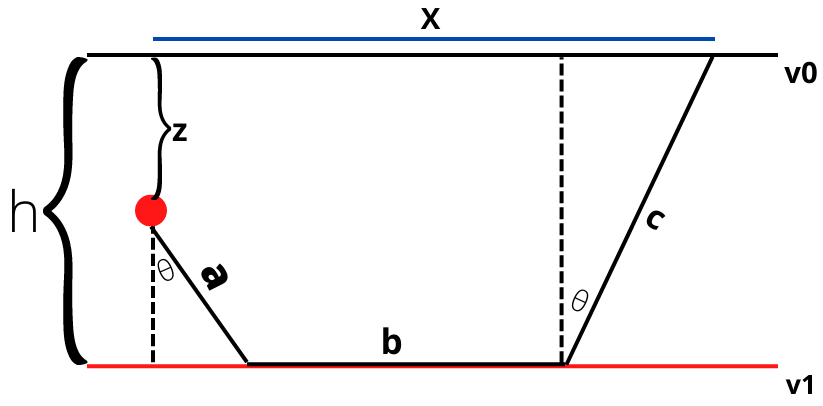
\includegraphics[width=\textwidth]{h.png}
	\caption{Representación gráfica del problema.}
\end{figure*}
se tienen las siguientes relaciones a partir de la ley de Snell:
\begin{align*}
	\frac{sin(\theta)}{v_0}&=\frac{1}{v_1} \implies sin(\theta)=\frac{v_0}{v_1}
	\\ v_1&=\frac{v_0}{sen(\theta )}
\end{align*}
y se sabe además, por trigonometría:
\begin{align*}
	a&=\frac{h-z}{cos(\theta )} \\
	b&= x-tan(\theta )(h-z)-tan(\theta)h=x-tan(\theta )(2h -z) \\
	c&=\frac{h}{cos(\theta )}
\end{align*}
y bien, el tiempo de llegada puede ser expresado por la suma que demora cada tramo, es decir:
\begin{equation*}
	T=\frac{a}{v_0}+\frac{b}{v_1}+\frac{c}{v_0}
\end{equation*}
Reemplazando:
\begin{align*}
	T&=\frac{\frac{h-z}{cos(\theta )}}{v_0}+\frac{x-tan(\theta )(2h -z)}{v_1}+\frac{\frac{h}{cos(\theta )}}{v_0} \\
	T&=\frac{x}{v_1}+ \frac{(2h-z)}{cos(\theta)v_0}-\frac{(2h-z)tan(\theta)}{v_1} \\ 
	T&=\frac{x}{v_1}+(2h-z)\left(\frac{1}{cos(\theta )v_0}-\frac{tan(\theta )}{v_1}\right) \\ 
	T&=\frac{x}{v_1}+(2h-z)\left(\frac{1}{cos(\theta )v_0}-\frac{\tan(\theta)\sen(\theta)}{v_0}\right) \\ 
	T&=\frac{x}{v_1}+(2h-z)\left(\frac{1}{cos(\theta )v_0}-\frac{sen^2(\theta )}{cos(\theta )v_0}\right) \\ 
	T&=\frac{x}{v_1}+(2h-z)\left(\frac{cos(\theta )}{v_0}\right) \\ 
	T&=\frac{x}{v_1}+(2h-z)\left(\sqrt{\frac{cos^2(\theta )}{v_0^2}}\right) \\
	T&=\frac{x}{v_1}+(2h-z)\left(\sqrt{\frac{1-sen^2(\theta )}{v_0^2}}\right) \\
	\Aboxed{T&=\frac{x}{v_1}+(2h-z)\left(\sqrt{\frac{1}{v_0^2}-\frac{1}{v_1^2}}\right)}
\end{align*}
Obteniendo una relación del tiempo respecto a $x, v_0,v_1,h$ y $z$. PD: el paso de pasar a raiz es debido a que el valor dentro es positivo siempre).
\end{document}